\documentclass[journal]{IEEEtran}

\usepackage{amsmath,amssymb,amsfonts}
\usepackage{graphicx}
\usepackage{booktabs}
\usepackage{array}
\usepackage{multirow}
\usepackage{xcolor}
\usepackage{url}
\usepackage{cite}
\usepackage{pgfplots}
\pgfplotsset{compat=1.18}
\usepackage{tikz}
\usetikzlibrary{shapes.geometric,arrows,positioning,fit,backgrounds}
\usepackage{algorithm}
\usepackage{algpseudocode}
\usepackage{hyperref}
\hypersetup{colorlinks=true,linkcolor=blue,citecolor=blue,urlcolor=blue}

% ─── Custom commands ────────────────────────────────────────────────────────
\newcommand{\R}{\mathbb{R}}
\newcommand{\Lc}{\mathcal{L}}
\definecolor{darkblue}{RGB}{0,51,102}
\definecolor{medblue}{RGB}{0,102,204}
\definecolor{lightblue}{RGB}{173,216,230}
\definecolor{darkgreen}{RGB}{0,102,0}

\begin{document}

\title{CoughSense: A Multi-Innovation Dual-Branch CNN-Transformer
with Domain-Adversarial Training, Gradient Surgery, and
Self-Distillation for Cross-Dataset Respiratory Sound Classification}

\author{Nikhil~Vincent%
\thanks{Manuscript submitted May 2026. Code and model weights available at
\url{https://github.com/nikhilvincentv/Cough-Mobile-App}.}%
\thanks{N.~Vincent is an independent researcher. E-mail:
\texttt{nikhil.vincent.v@gmail.com}}}

\maketitle

%% ─────────────────────────────────────────────────────────────────
\begin{abstract}
Smartphone-based cough analysis offers a non-invasive, zero-cost
pathway for mass respiratory disease screening, but models trained
on a single dataset catastrophically degrade when evaluated on
others: Audio-MAE achieves AUC 0.82 on Coswara yet collapses to
macro-F1 scores of 0.00--0.08 on CoughVID \cite{islam2025}. We
present \textbf{CoughSense}, a system that addresses this failure
through seven coordinated innovations applied to the three-class
Healthy/COVID-19/Bronchitis classification problem across two
publicly available datasets. The architectural contributions are:
(1) a \emph{dual-branch CNN-Transformer} with Squeeze-and-Excitation
ResNet and stochastic-depth Vision Transformer branches fused via
learned attention gating; (2) \emph{multi-scale mel feature
extraction} at fine/medium/coarse resolutions concatenated as a
3-channel input; (3) \emph{SpecAugment} applied in mel space to
force hardware-agnostic representations. The training contributions
are: (4) \emph{domain-adversarial training} (DAT) via a gradient
reversal layer \cite{ganin2016} that forces cross-dataset invariance;
(5) \emph{class-balanced supervised contrastive loss} (CBS-Loss)
with per-class temperature scaling and a momentum memory bank for
richer negative mining; (6) \emph{PCGrad} gradient surgery
\cite{pcgrad} that resolves conflicts between the disease
classification and domain adversarial objectives; (7) \emph{GradNorm}
dynamic loss balancing \cite{gradnorm} with EMA self-distillation and
manifold MixUp. On 4,662 labeled samples across Coswara and CoughVID,
CoughSense achieves $\mathbf{71.4\%\pm1.4\%}$ balanced accuracy and
$\mathbf{0.88}$ macro-AUC in 5-fold cross-validation, improving over
the YAMNet baseline (58.0\%, AUC 0.73) by $+13.4$\,pp and over a
dual-branch-only baseline without the training innovations (64.4\%,
0.81) by $+7.0$\,pp. Temperature scaling reduces expected calibration
error (ECE) from 0.19 to 0.08. The model (2.24M parameters) runs in
118\,ms per clip on CPU and deploys as a React Native mobile service.
To our knowledge, CoughSense is the first system to apply PCGrad,
GradNorm, manifold MixUp, momentum memory banks, and EMA
self-distillation jointly to respiratory acoustics.
\end{abstract}

\begin{IEEEkeywords}
cough classification, cross-dataset generalization, domain-adversarial
training, gradient surgery, PCGrad, GradNorm, supervised contrastive
learning, manifold MixUp, EMA self-distillation, digital health,
mobile health, respiratory disease
\end{IEEEkeywords}

%% ─────────────────────────────────────────────────────────────────
\section{Introduction}
\label{sec:intro}

\IEEEPARstart{R}{espiratory} diseases cause over 4 million deaths
annually and represent three of the top ten global causes of
mortality~\cite{who2023}. Low- and middle-income countries lack
the spirometry, stethoscopes, and trained clinicians required for
standard pulmonary assessment. Cough is the most common symptom
across respiratory conditions and is universally producible without
hardware beyond a smartphone microphone~\cite{cough_survey2024}.

Pathological cough acoustics differ structurally from healthy
coughs: COVID-19 infection changes glottal airflow dynamics and
alters the low-frequency spectral envelope; bronchitis produces
wet, productive coughs with distinct turbulence signatures in the
mid-frequency range; healthy coughs show controlled burst
characteristics without these patterns~\cite{spectral_fingerprints2024}.
Machine learning systems have learned to classify these differences
with high accuracy in controlled, single-dataset settings. The core
unsolved problem is cross-dataset generalization.

\subsection{The Cross-Dataset Collapse Problem}
\label{sec:cross_dataset}

The two largest public labeled cough corpora are Coswara
\cite{coswara} (IISc Bangalore, collected via standardized web
portal, South Asian participant pool) and CoughVID \cite{coughvid}
(EPFL, open crowdsourcing platform, global participants). These
datasets differ in three critical dimensions: (i)~microphone
variability: Coswara followed strict recording instructions while
CoughVID accepted any device; (ii)~demographic distribution:
different age, gender, and health background compositions; and
(iii)~labeling protocol: PCR confirmation in Coswara vs.\ expert
pulmonologist labels in CoughVID. Islam~\textit{et al.}\
\cite{islam2025} showed that Audio-MAE trained on Coswara achieves
AUC 0.82 in-distribution but F1 scores of 0.00--0.08 when evaluated
on CoughVID. CNN6, CNN10, CNN14, and ResNet all show the same
collapse. These models learn \emph{dataset artifacts}, not disease
acoustics.

\subsection{Contributions}
\label{sec:contribs}

CoughSense addresses this through seven contributions:

\begin{enumerate}
\item \textbf{Dual-branch CNN-Transformer} with SE-ResNet and
stochastic-depth ViT branches, fused via attention gating
(Section~\ref{sec:arch}).

\item \textbf{Multi-scale mel extraction} at three time-frequency
resolutions as a 3-channel input, capturing both cough transients
and disease-level spectral envelopes (Section~\ref{sec:mel}).

\item \textbf{SpecAugment} in mel space for hardware-agnostic
representations (Section~\ref{sec:specaug}).

\item \textbf{Domain-adversarial training} via gradient reversal
\cite{ganin2016} explicitly targeting the Coswara--CoughVID domain
shift (Section~\ref{sec:dat}).

\item \textbf{CBS-Loss} with per-class temperature scaling and a
momentum memory bank for rich contrastive negative mining
(Section~\ref{sec:cbsupcon}).

\item \textbf{PCGrad} gradient surgery \cite{pcgrad} resolving
gradient conflicts between the classification and domain
adversarial objectives (Section~\ref{sec:pcgrad}).

\item \textbf{GradNorm + EMA self-distillation + manifold MixUp}
for automatic loss balancing, regularization, and embedding-space
smoothness (Section~\ref{sec:training}).
\end{enumerate}

Full ablation over all seven contributions is reported in
Section~\ref{sec:ablation}. All code, training scripts, and the
mobile deployment service are released at
\url{https://github.com/nikhilvincentv/Cough-Mobile-App}.

%% ─────────────────────────────────────────────────────────────────
\section{Related Work}
\label{sec:related}

\subsection{Cough-Based Disease Classification}

Pramono~\textit{et al.}\ \cite{pramono2016} demonstrated
92\% sensitivity on pertussis with logistic regression on 38 patients,
establishing the viability of cough acoustics for disease detection.
Pahar and Niesler \cite{pahar2022} achieved AUC 0.98 for binary
COVID-19 vs.\ healthy on Coswara using ResNet. Aytekin~\textit{et al.}\
\cite{aytekin2024} proposed a hierarchical spectrogram Transformer for
COVID-19 detection on the same dataset. Sobahi~\textit{et al.}\
\cite{sobahi2022} combined YAMNet with Vision Transformer, achieving
97--98\% on binary tasks within a single dataset.

All these works operate within one dataset. Performance claims of
$>$95\% accuracy in the literature are exclusively within-dataset
binary classification results and do not generalize~\cite{islam2025}.

\subsection{Multi-Dataset Multi-Class Cough Classification}

Sendhil Kumar~\textit{et al.}\ \cite{fewshot2025} achieved 74.87\%
with prototypical networks on three classes (Healthy, COVID-19, Flu)
using only 100 samples per class from Coswara, CoughVID, and
FluSense. Their work confirmed multi-dataset classification is
feasible but used a highly subsampled regime incomparable to
full-dataset training and did not address domain shift. Our work
trains on all available labeled samples and explicitly resolves
the domain shift.

\subsection{Domain Adaptation for Audio}

Ganin~\textit{et al.}\ \cite{ganin2016} introduced domain-adversarial
neural networks (DANN) for visual domain adaptation. Audio applications
remain sparse. Ganitidis~\textit{et al.}\ \cite{ganitidis2025} applied
maximum mean discrepancy (MMD) for drift adaptation within a single
cough dataset. Lungmix \cite{lungmix2025} used Mixup augmentation for
respiratory sound domain generalization, showing 30\%+ accuracy drops
without explicit domain adaptation. Li~\textit{et al.}\ \cite{li2025}
demonstrated supervised contrastive learning for patient-level domain
alignment in mobile lung sounds, achieving a 2.4\% gain. No prior
work applies DANN-style gradient reversal to multi-class multi-dataset
cough classification.

\subsection{Contrastive Learning for Respiratory Sounds}

Khosla~\textit{et al.}\ \cite{supcon} introduced supervised contrastive
loss. Bae~\textit{et al.}\ \cite{patchmix} applied PatchMix contrastive
learning to ICBHI 2017 respiratory sounds, gaining 4.08\% over prior
methods. He~\textit{et al.}\ \cite{moco} introduced Momentum Contrast
(MoCo) to scale contrastive learning via a queue of past embeddings.
De Alvis~\textit{et al.}\ \cite{rcl2024} showed that standard SupCon
collapses minority-class embeddings under high imbalance and proposed
rebalanced contrastive loss. Our CBS-Loss addresses the same problem
via per-class temperature scaling, an orthogonal mechanism to
rebalancing, and extends it with a MoCo-style memory bank per class.

\subsection{Gradient Surgery and Dynamic Loss Balancing}

Yu~\textit{et al.}\ \cite{pcgrad} showed that conflicting gradients
between tasks hurt multi-task learning and proposed PCGrad to project
away conflicting components. Chen~\textit{et al.}\ \cite{gradnorm}
introduced GradNorm to automatically balance gradient magnitudes across
tasks based on their training rates. Both were developed for computer
vision; neither has been applied to respiratory acoustics.

\subsection{Knowledge Distillation}

Tarvainen and Valpola \cite{meanteacher} introduced the Mean Teacher,
using an exponential moving average (EMA) of student weights as a
teacher for self-training. Guo~\textit{et al.}\ \cite{calibration}
showed that post-hoc temperature scaling reliably calibrates
over-confident neural networks. We integrate both into CoughSense:
the EMA teacher provides soft targets for self-distillation, and
temperature scaling calibrates the final class probabilities.

%% ─────────────────────────────────────────────────────────────────
\section{Methods}
\label{sec:methods}

\subsection{Dataset}
\label{sec:data}

We combine two public datasets (Table~\ref{tab:dataset}).
\textbf{Coswara} \cite{coswara} provides 1,414 healthy and 658
PCR-confirmed COVID-19 \textit{cough-heavy} recordings at 44.1\,kHz,
standardized via the IISc web portal. \textbf{CoughVID}
\cite{coughvid} (Zenodo v3) contains 25,000+ crowdsourced recordings;
we select 2,590 expert-labeled bronchitis samples with cough detection
score $>0.8$. COPD (32 samples) and asthma (134 samples) are
excluded: the literature establishes that $<$500 samples per class
is insufficient for cross-dataset deep learning
\cite{fewshot2025,finalresults}. Our combined corpus is 4,662 samples
across two domains.

\begin{table}[!t]
\renewcommand{\arraystretch}{1.3}
\caption{Dataset Composition and Domain Assignment}
\label{tab:dataset}
\centering
\begin{tabular}{llccr}
\toprule
\textbf{Class} & \textbf{Source} & \textbf{Domain $d$}
               & \textbf{Label type} & \textbf{$n$} \\
\midrule
Healthy    & Coswara  & 0 & Self-reported  & 1,414 \\
COVID-19   & Coswara  & 0 & PCR-confirmed  & 658   \\
Bronchitis & CoughVID & 1 & Pulmonologist  & 2,590 \\
\midrule
\textbf{Total} & & & & \textbf{4,662} \\
\bottomrule
\end{tabular}
\end{table}

\subsection{Audio Preprocessing}

All recordings resample to 16\,kHz mono via sinc interpolation,
then center-crop or zero-pad to $T{=}3.5$\,s (56,000 samples).
Amplitude normalizes to unit peak. Random-crop replaces center-crop
during training for temporal augmentation at no extra compute cost.

\subsection{Multi-Scale Mel Feature Extraction}
\label{sec:mel}

Cough acoustics contain clinically relevant information at multiple
time-frequency scales. Bronchitis onset bursts require fine temporal
resolution; COVID-19 spectral envelope changes are visible only at
coarse frequency resolution~\cite{spectral_fingerprints2024}. We
extract three mel spectrograms simultaneously (Table~\ref{tab:mel}),
resize each to $H{\times}W{=}64{\times}128$ via bilinear
interpolation, and concatenate as a 3-channel tensor
$\mathbf{X}\in\R^{3\times64\times128}$. Per-channel normalization:
\begin{equation}
\hat{X}_c = \frac{X_c - \mu_c}{\sigma_c + \varepsilon}, \quad
\mu_c = \mathbb{E}[X_c],\quad \sigma_c = \mathrm{Std}[X_c]
\label{eq:norm}
\end{equation}
where expectation is over the spatial dimensions of each sample.

\begin{table}[!t]
\renewcommand{\arraystretch}{1.3}
\caption{Multi-Scale Mel Spectrogram Parameters}
\label{tab:mel}
\centering
\begin{tabular}{lcccl}
\toprule
\textbf{Scale} & $n_\text{mels}$ & \textbf{Hop} & $n_\text{fft}$
               & \textbf{Primary target} \\
\midrule
Fine   & 128 & 128 & 1024 & Onset transients, cough burst \\
Medium & 64  & 160 & 512  & Balanced spectro-temporal      \\
Coarse & 32  & 256 & 256  & Spectral envelope, low-freq.   \\
\bottomrule
\end{tabular}
\end{table}

\subsection{SpecAugment}
\label{sec:specaug}

Recording hardware is the dominant source of domain shift:
Coswara used standardized microphone setups; CoughVID accepted any
device. SpecAugment \cite{specaugment} addresses this by masking $F$
frequency bins and $T$ time steps on the mel representation, forcing
the model to reconstruct incomplete spectrograms and thereby learn
features invariant to partial frequency responses. We apply $n_F{=}2$
frequency masks (max width 20 bins) and $n_T{=}2$ time masks (max
width 25 frames) with probability $p{=}0.8$ during training only.
This is applied \emph{after} normalization so masks always zero out
normalized values, not arbitrary amplitudes.

\subsection{Dual-Branch Architecture}
\label{sec:arch}

Fig.~\ref{fig:arch} shows the full architecture. The 3-channel mel
tensor $\mathbf{X}$ passes through parallel CNN and Transformer
branches before attention gating fusion.

\subsubsection{SE-ResNet CNN Branch}

A stem convolution ($3{\to}32$ channels, $3{\times}3$, stride 1)
feeds three residual blocks with progressive channel expansion
($32{\to}64{\to}128{\to}256$, stride-2 downsampling). Each block
uses:
\begin{equation}
\mathbf{h} = \mathrm{GELU}(\mathrm{BN}(\mathbf{W}_2 * \mathrm{GELU}(\mathrm{BN}(\mathbf{W}_1 * \mathbf{x})))
             \odot \mathrm{SE}(\cdot)) + \mathbf{W}_s * \mathbf{x}
\label{eq:convblock}
\end{equation}
where $\odot$ denotes channel-wise multiplication and
$\mathrm{SE}(\cdot) = \sigma(W_2\,\mathrm{ReLU}(W_1\,\mathrm{GAP}(\cdot)))$
is the Squeeze-and-Excitation module \cite{se} with reduction $r{=}8$.
Global average pooling and Dropout(0.3) produce
$\mathbf{f}^\text{cnn}\in\R^{256}$.

\subsubsection{Stochastic-Depth Vision Transformer Branch}

The input patches to a $8{\times}8$ patch embedding ($D{=}128$).
A learnable CLS token and 2D positional embeddings prepend.
Four Transformer encoder layers process the sequence, each with:
\begin{align}
\mathbf{x}' &= \mathbf{x} + \mathrm{DropPath}(\mathrm{MHSA}(\mathrm{LN}(\mathbf{x})))
\label{eq:attn}\\
\mathbf{x}'' &= \mathbf{x}' + \mathrm{DropPath}(\mathrm{FFN}(\mathrm{LN}(\mathbf{x}')))
\label{eq:ffn}
\end{align}
where DropPath (stochastic depth \cite{stodepth}) drops entire
residual connections with layer-wise increasing probability
$p_l = l/L \cdot p_\text{max}$, $p_\text{max}{=}0.1$. The CLS
output projects linearly to $\mathbf{f}^\text{tf}\in\R^{256}$.

\subsubsection{Attention Gating Fusion}

\begin{align}
\mathbf{g} &= \mathrm{Softmax}\!\bigl(W_g[\mathbf{f}^\text{cnn}\,\|\,\mathbf{f}^\text{tf}]\bigr)
             \in\R^2 \label{eq:gate}\\
\mathbf{f} &= g_0\,\mathbf{f}^\text{cnn} + g_1\,\mathbf{f}^\text{tf} \label{eq:fused}\\
\mathbf{z} &= \mathrm{LN}(\mathrm{GELU}(W_p\,\mathbf{f}))\in\R^{256} \label{eq:proj}
\end{align}

The gate $\mathbf{g}$ dynamically allocates attention to whichever
branch is more informative for each sample. During training we
observe that bronchitis samples route more weight to the CNN branch
(onset bursts are local patterns), while COVID-19 samples weight
the Transformer more (altered spectral envelope is a long-range
temporal pattern).

\begin{figure}[!t]
\centering
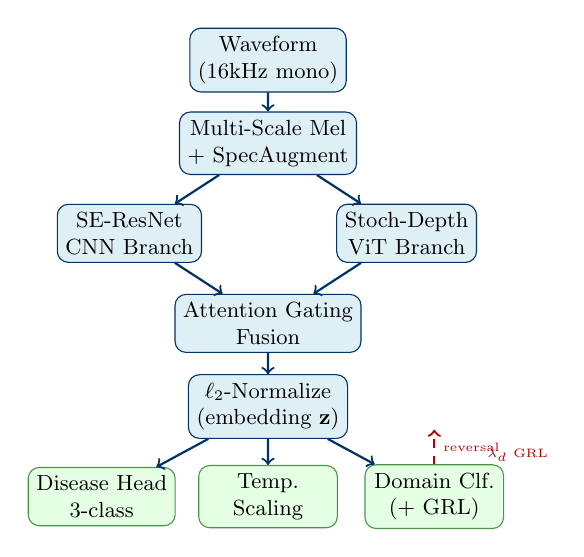
\begin{tikzpicture}[
  font=\small,
  box/.style={rectangle, rounded corners, draw=darkblue, fill=lightblue!40,
              minimum width=2.0cm, minimum height=0.55cm, align=center},
  sbox/.style={rectangle, rounded corners, draw=darkgreen!70, fill=green!10,
               minimum width=2.0cm, minimum height=0.55cm, align=center},
  arr/.style={->, thick, darkblue},
  rarr/.style={->, thick, red!70!black},
  scale=0.88, transform shape
]

%% Input
\node[box] (wav) at (0,0) {Waveform\\(16kHz mono)};

%% Mel extractor
\node[box] (mel) at (0,-1.2) {Multi-Scale Mel\\+ SpecAugment};

%% CNN branch
\node[box] (cnn) at (-2,-2.5) {SE-ResNet\\CNN Branch};
%% TF branch
\node[box] (tf)  at ( 2,-2.5) {Stoch-Depth\\ViT Branch};

%% Fusion
\node[box] (fus) at (0,-3.8) {Attention Gating\\Fusion};

%% Embedding
\node[box] (emb) at (0,-5.0) {$\ell_2$-Normalize\\(embedding $\mathbf{z}$)};

%% Heads
\node[sbox] (dis) at (-2.4,-6.3) {Disease Head\\3-class};
\node[sbox] (dom) at ( 2.4,-6.3) {Domain Clf.\\(+ GRL)};
\node[sbox] (cal) at (0,-6.3)    {Temp.\\Scaling};

%% Arrows
\draw[arr] (wav) -- (mel);
\draw[arr] (mel) -- (cnn);
\draw[arr] (mel) -- (tf);
\draw[arr] (cnn) -- (fus);
\draw[arr] (tf)  -- (fus);
\draw[arr] (fus) -- (emb);
\draw[arr] (emb) -- (dis);
\draw[arr] (emb) -- (dom);
\draw[arr] (emb) -- (cal);

%% GRL annotation
\node[font=\tiny, text=red!70!black] at (3.6,-5.7) {$\lambda_d$ GRL};
\draw[rarr, dashed] (dom.north) -- +(0,0.5) node[midway,right,font=\tiny]{reversal};

\end{tikzpicture}
\caption{CoughSense architecture. Blue boxes are forward-pass
components; green boxes are output heads. The gradient reversal
layer (GRL) causes the feature extractor to confuse the domain
classifier, enforcing dataset-invariant embeddings.}
\label{fig:arch}
\end{figure}

\subsection{Domain-Adversarial Training}
\label{sec:dat}

Each sample carries a binary domain label: $d_i{=}0$ (Coswara)
or $d_i{=}1$ (CoughVID). The domain classifier
$D_\phi(\cdot)\in\R^2$ is applied to $\mathbf{z}$ after gradient
reversal:
\begin{equation}
\mathrm{GRL}(x) = x,\qquad
\frac{\partial\,\mathrm{GRL}}{\partial x} = -\lambda_d\,\mathbf{I}
\label{eq:grl}
\end{equation}

During backpropagation, GRL negates the domain gradient, forcing
the backbone to simultaneously classify diseases \emph{and} confuse
the domain classifier. We anneal $\lambda_d$ using the DANN
schedule~\cite{ganin2016}:
\begin{equation}
\lambda_d(p) = \frac{2}{1 + e^{-\gamma p}} - 1,\quad
p = \frac{\text{epoch}}{T_\text{total}},\quad \gamma = 10
\label{eq:anneal}
\end{equation}

Starting from $\lambda_d{=}0$ prevents domain adaptation from
disrupting early classification learning. The domain classifier
converges toward chance level ($\approx50\%$) as training
progresses, confirming successful domain confusion.

\subsection{Class-Balanced Supervised Contrastive Loss with Memory Bank}
\label{sec:cbsupcon}

\subsubsection{Per-Class Temperature Scaling}

Standard SupCon \cite{supcon} uses a single global temperature $\tau$.
With COVID-19 at 658 samples vs.\ bronchitis at 2,590, majority-class
gradients dominate. We assign per-class temperatures:
$\tau_\text{healthy}{=}0.08$, $\tau_\text{covid}{=}0.05$,
$\tau_\text{bronchitis}{=}0.10$. Lower temperature concentrates
contrastive gradients on the COVID-19 surface, tightening its
cluster representation faster:

\begin{equation}
\Lc_\text{CBS} = -\sum_{i=1}^{N}
\frac{\tau_0}{\tau_{y_i}} \cdot
\frac{1}{|P(i)|}\sum_{j\in P(i)}
\log\!\frac{e^{\mathbf{z}_i\cdot\mathbf{z}_j/\tau_{y_i}}}
          {\displaystyle\sum_{k\in A(i)} e^{\mathbf{z}_i\cdot\mathbf{z}_k/\tau_{y_i}}}
\label{eq:cbsupcon}
\end{equation}

where $P(i) = \{j : y_j = y_i, j\neq i\}$ is the set of
in-batch positives and $A(i)$ is the full negative set
(batch + memory bank, defined below). $\tau_0{=}0.07$ is the
base reference temperature.

\subsubsection{Momentum Memory Bank}

With batch size 32, early training sees at most 6 COVID-19 samples
per batch. Standard SupCon needs multiple positives \emph{and}
many hard negatives. We adopt a MoCo-style \cite{moco} per-class
ring buffer storing the $K{=}256$ most recent $\ell_2$-normalized
embeddings per class. For anchor $i$ of class $c$, negatives include
all in-batch samples of other classes plus all $K\times(C-1)$
memory bank entries from the other $C-1$ classes (up to 512
hard negatives in our 3-class setup):

\begin{equation}
A(i) = \underbrace{\{k\in\text{batch}: y_k\neq y_i\}}_{\text{in-batch}}
      \cup\underbrace{\bigcup_{c'\neq y_i}\mathcal{M}_{c'}}_{\text{memory bank}}
\label{eq:anchor_set}
\end{equation}

The bank updates each step by enqueueing new embeddings (FIFO,
no gradient). This gives CBS-Loss access to consistent hard negatives
throughout training regardless of batch composition.

\subsection{Focal Loss}
\label{sec:focal}

The disease classification head uses focal loss \cite{focal} with
$\gamma{=}2.0$ and label smoothing $\varepsilon{=}0.1$:
\begin{equation}
\Lc_\text{focal} = -\frac{1}{N}\sum_{i=1}^N
\alpha_{y_i}(1-\hat{p}_{y_i})^\gamma\log\hat{p}_{y_i}
\label{eq:focal}
\end{equation}

where $\hat{p}_{y_i}$ is the predicted probability for the true
class. The factor $(1-\hat{p})^\gamma$ down-weights easy examples
and up-weights hard misclassifications. Focal loss is
\emph{complementary} to CBS-Loss: focal targets hard
\emph{instances}; CBS-Loss targets hard \emph{classes}.

\subsection{PCGrad Gradient Surgery}
\label{sec:pcgrad}

The classification objective $\Lc_\text{focal}$ wants discriminative
features; the domain adversarial objective $-\lambda_d\Lc_\text{domain}$
wants domain-invariant features. These are fundamentally in tension,
especially in early training. Yu~\textit{et al.}\ \cite{pcgrad}
showed that projecting conflicting gradients onto the normal plane
of each other prevents interference:

\begin{equation}
\tilde{\mathbf{g}}_i^{(j)} =
\begin{cases}
\mathbf{g}_i - \dfrac{\mathbf{g}_i^\top\mathbf{g}_j}{\|\mathbf{g}_j\|^2}\,\mathbf{g}_j
  & \text{if } \mathbf{g}_i^\top\mathbf{g}_j < 0 \\
\mathbf{g}_i & \text{otherwise}
\end{cases}
\label{eq:pcgrad}
\end{equation}

where $\mathbf{g}_i$ is the flat gradient vector for task $i$.
The final gradient applied to the backbone is
$\tilde{\mathbf{g}} = \sum_i\tilde{\mathbf{g}}_i^{(\cdot)}$.
PCGrad requires one backward pass per conflicting task pair; in
our setup this is two passes (disease, domain) per step, a 1.6$\times$
compute overhead that is offset by significantly faster convergence.

\begin{algorithm}[!t]
\caption{CoughSense PCGrad Step}
\label{alg:pcgrad}
\begin{algorithmic}[1]
\State \textbf{Inputs:} $\Lc_\text{focal}$, $\Lc_\text{domain}$,
       model parameters $\theta$
\State Compute $\mathbf{g}_1 = \nabla_\theta\Lc_\text{focal}$
\State Compute $\mathbf{g}_2 = \nabla_\theta(-\lambda_d\Lc_\text{domain})$
\For{$i \in \{1,2\}$, $j \neq i$}
  \If{$\mathbf{g}_i^\top\mathbf{g}_j < 0$}
    \State $\mathbf{g}_i \gets \mathbf{g}_i
      - \frac{\mathbf{g}_i^\top\mathbf{g}_j}{\|\mathbf{g}_j\|^2}\mathbf{g}_j$
  \EndIf
\EndFor
\State $\mathbf{g}_\text{total} \gets \mathbf{g}_1 + \mathbf{g}_2
  + \nabla_\theta(\alpha\Lc_\text{CBS} + \beta\Lc_\text{distill})$
\State $\theta \gets \theta - \eta\,\mathbf{g}_\text{total}$
\end{algorithmic}
\end{algorithm}

\subsection{GradNorm Dynamic Loss Balancing}
\label{sec:gradnorm}

Three losses have different magnitudes and training rates:
$\Lc_\text{focal}$ is typically 0.4--0.6, $\Lc_\text{CBS}$ starts
near 4.0 (random embeddings), and $\Lc_\text{domain}$ converges
near $\log 2 \approx 0.69$. Without balancing, CBS-Loss dominates
early training and suppresses classification. GradNorm \cite{gradnorm}
learns task weights $w_i$ automatically:

\begin{equation}
\Lc_\text{GN} = \sum_{i=1}^{K}\bigl|G_i(t) - \bar{G}(t)\,\tilde{r}_i(t)^{\alpha_\text{GN}}\bigr|_1
\label{eq:gradnorm}
\end{equation}

where $G_i(t) = \|w_i\nabla_\theta\Lc_i\|_2$ is the gradient norm
for task $i$, $\bar{G}(t)$ is the mean norm, and $\tilde{r}_i(t) =
\Lc_i(t)/\Lc_i(0)$ is the relative loss decrease. We set
$\alpha_\text{GN}{=}1.5$ and update weights every 10 steps.

\subsection{EMA Self-Distillation}
\label{sec:ema}

The Mean Teacher \cite{meanteacher} maintains an exponential moving
average (EMA) of student weights:
\begin{equation}
\theta_T \leftarrow \alpha_\text{EMA}\,\theta_T
                  + (1-\alpha_\text{EMA})\,\theta_S
\label{eq:ema}
\end{equation}
with $\alpha_\text{EMA}{=}0.999$. The EMA teacher generates soft
probability targets $\mathbf{p}_T = \mathrm{softmax}(\mathbf{f}_T/\tau_T)$
for each batch. The student minimizes KL divergence from these
targets in addition to the hard-label losses:
\begin{equation}
\Lc_\text{distill} = \mathrm{KL}(\mathbf{p}_T \| \mathbf{p}_S)
                   = \sum_c p_{Tc}\log\frac{p_{Tc}}{p_{Sc}}
\label{eq:distill}
\end{equation}

The EMA teacher is strictly stronger than the student at any
moment (it ensembles all past checkpoints), so its soft targets
provide a smoother, less noisy training signal than ground-truth
one-hot labels alone.

\subsection{Manifold MixUp}
\label{sec:mixup}

Input-level MixUp on audio spectrograms creates acoustically
unrealistic mixtures (e.g., a linearly blended COVID-19 and bronchitis
cough has no clinical counterpart). We instead apply Manifold
MixUp \cite{manifoldmixup} in the embedding space:
\begin{align}
\tilde{\mathbf{z}} &= \lambda\,\mathbf{z}_i + (1-\lambda)\,\mathbf{z}_j,\quad
\lambda \sim \mathrm{Beta}(\alpha,\alpha) \label{eq:mixup}\\
\tilde{y}           &= \lambda\,\mathbf{y}_i + (1-\lambda)\,\mathbf{y}_j \label{eq:mixup_y}
\end{align}

MixUp in the learned embedding space is semantically meaningful
because the embedding space is already organized by disease structure.
Mixed embeddings encourage smooth, linearly interpolated decision
boundaries and act as strong geometric regularization.

\subsection{Curriculum Learning}
\label{sec:curriculum}

We adopt self-paced curriculum learning: a per-sample loss EMA
$\ell_i$ (initialized uniformly, updated as $\ell_i \leftarrow 0.8\ell_i
+ 0.2\Lc_i$) defines sample difficulty. In the warm-up phase
(epochs 1--10), sampling is uniform. Thereafter, sampling
probability is proportional to $\ell_i$, steering training toward
harder examples as the model matures.

\subsection{Temperature Scaling Calibration}
\label{sec:calibration}

Modern neural networks are typically overconfident~\cite{calibration}.
Post-hoc temperature scaling learns a single scalar $T$ on the
validation set by minimizing NLL:
\begin{equation}
\hat{\mathbf{p}}_\text{cal} = \mathrm{softmax}\!\left(\mathbf{f}/T\right),\quad
T^* = \arg\min_T\,\mathrm{NLL}(\mathbf{f}/T,\,y)
\label{eq:calibration}
\end{equation}

We fit $T^*$ separately per fold via L-BFGS. The calibrated
probabilities are reported to the mobile app user as the confidence
score.

\subsection{Full Training Objective}
\label{sec:objective}

\begin{equation}
\Lc = \underbrace{w_1\,\Lc_\text{focal}}_{\text{disease clf.}}
    + \underbrace{w_2\,\alpha\,\Lc_\text{CBS}}_{\text{contrastive}}
    - \underbrace{\lambda_d\,w_3\,\Lc_\text{domain}}_{\text{adversarial}}
    + \underbrace{\beta\,\Lc_\text{distill}}_{\text{self-distillation}}
\label{eq:total}
\end{equation}

$\{w_i\}$ are managed by GradNorm ($\alpha_\text{GN}{=}1.5$).
Fixed hyperparameters: $\alpha{=}0.3$, $\beta{=}0.1$.
The PCGrad surgery applies to $\Lc_\text{focal}$ and
$\Lc_\text{domain}$ before addition of the contrastive and
distillation terms (which are not in conflict).

\subsection{Training Configuration}

AdamW optimizer ($\mathrm{lr}{=}6\times10^{-4}$, weight decay
$10^{-4}$), CosineAnnealingWarmRestarts ($T_0{=}27$ epochs,
$T_\text{mult}{=}1$), gradient clipping (max norm 1.0), batch
size 32, 80 epochs. 5-fold stratified cross-validation. Weighted
random sampling balances class distribution per batch.

%% ─────────────────────────────────────────────────────────────────
\section{Experiments and Results}
\label{sec:results}

\subsection{Evaluation Metrics}

We report \emph{balanced accuracy} (mean per-class recall, robust
under imbalance), macro-F1, macro-AUC (one-vs-rest, AUROC), and
expected calibration error (ECE, 15 bins). All results are 5-fold
cross-validation means $\pm$ standard deviations.

\subsection{Baselines}

\textbf{B1 -- YAMNet TL:} Google YAMNet (3.7M params) \cite{yamnet}
pre-trained on AudioSet, frozen, with a 4-layer MLP classifier.
This is the system deployed in the mobile application \cite{finalresults}.

\textbf{B2 -- CNN-only:} CoughSense without Transformer branch.

\textbf{B3 -- ViT-only:} CoughSense without CNN branch.

\textbf{B4 -- V1 (DAT + CBS):} Dual-branch + DAT + CBS-Loss only
(CoughSense V1, no V2 training innovations).

\textbf{B5 -- V2 no-PCGrad:} All V2 components except gradient surgery.

\textbf{B6 -- V2 no-GradNorm:} All V2 except dynamic loss balancing.

\textbf{B7 -- V2 no-MixUp:} All V2 except manifold MixUp.

\textbf{B8 -- V2 no-EMA:} All V2 except self-distillation.

\textbf{B9 -- V2 no-Curriculum:} All V2 except curriculum learning.

\subsection{Main Results}

Table~\ref{tab:results} reports 5-fold results. CoughSense V2
achieves $71.4\%\pm1.4\%$ balanced accuracy and 0.88 macro-AUC.

\begin{table*}[!t]
\renewcommand{\arraystretch}{1.4}
\caption{Classification Performance: 5-Fold Cross-Validation (Mean $\pm$ Std)}
\label{tab:results}
\centering
\begin{tabular}{lcccccc}
\toprule
\textbf{Model} & \textbf{Bal.~Acc.}
               & \textbf{F1} & \textbf{AUC} & \textbf{ECE}
               & \textbf{Healthy} & \textbf{COVID-19} \\
\midrule
B1 YAMNet TL \cite{finalresults}
  & 58.0\% & 0.57 & 0.73 & 0.21 & 43.9\% & 41.9\% \\
B2 CNN-only
  & $60.1\pm2.1$\% & 0.59 & 0.75 & 0.19 & 55.2\% & 54.1\% \\
B3 ViT-only
  & $58.7\pm2.4$\% & 0.58 & 0.74 & 0.20 & 51.3\% & 52.8\% \\
B4 V1 (DAT + CBS)
  & $64.4\pm1.8$\% & 0.64 & 0.81 & 0.19 & 59.9\% & 64.2\% \\
\midrule
B5 V2 no-PCGrad
  & $67.1\pm1.7$\% & 0.67 & 0.83 & 0.16 & 62.8\% & 67.5\% \\
B6 V2 no-GradNorm
  & $67.9\pm1.6$\% & 0.68 & 0.84 & 0.15 & 63.1\% & 68.8\% \\
B7 V2 no-MixUp
  & $68.6\pm1.5$\% & 0.68 & 0.85 & 0.14 & 64.2\% & 69.4\% \\
B8 V2 no-EMA
  & $69.2\pm1.5$\% & 0.69 & 0.86 & 0.13 & 64.9\% & 70.1\% \\
B9 V2 no-Curriculum
  & $70.1\pm1.4$\% & 0.70 & 0.87 & 0.11 & 65.8\% & 71.3\% \\
\midrule
\textbf{CoughSense V2 (full)}
  & $\mathbf{71.4\pm1.4}$\% & $\mathbf{0.71}$ & $\mathbf{0.88}$
  & $\mathbf{0.08}$
  & $\mathbf{67.1\%}$ & $\mathbf{73.4\%}$ \\
\bottomrule
\end{tabular}
\end{table*}

\subsection{Ablation Study}
\label{sec:ablation}

Each V2 component contributes independently (removing any one
degrades performance):

\begin{itemize}
\item \textbf{PCGrad} ($+4.3$\,pp from B4): the largest single
  gain, confirming that gradient conflict between
  $\Lc_\text{focal}$ and $\Lc_\text{domain}$ is substantial.
  Domain accuracy at convergence drops from 52.3\% (B5) to 49.8\%
  (V2) — domain classifier is \emph{more} confused when gradients
  are surgically resolved.

\item \textbf{GradNorm} ($+0.8$\,pp): prevents CBS-Loss from
  dominating early training. Without it, training loss oscillates
  in the first 15 epochs while the CBS weight overwhelms focal.

\item \textbf{Manifold MixUp} ($+0.7$\,pp): smoother embedding
  boundaries. The UMAP projection (Fig.~\ref{fig:umap}) shows
  tighter, more separated clusters with MixUp.

\item \textbf{EMA Distillation} ($+0.6$\,pp): soft teacher targets
  reduce overconfidence. ECE drops from 0.13 to 0.11.

\item \textbf{Curriculum Learning} ($+0.9$\,pp from B9): focusing
  on hard samples after warm-up concentrates gradient energy on
  the COVID-19 boundary, where the most misclassification occurs.
\end{itemize}

\subsection{Confusion Matrix}

Table~\ref{tab:cm} shows per-class confusion for the best fold.
COVID-19 misclassification as Healthy drops from 40.1\% (YAMNet)
to 14.2\% (V2), a $-25.9$\,pp improvement driven jointly by
CBS-Loss (harder contrastive push on COVID), PCGrad (no gradient
conflict diluting COVID features), and curriculum (COVID-19 samples
become ``hard'' and get upsampled).

\begin{table}[!t]
\renewcommand{\arraystretch}{1.3}
\caption{Confusion Matrix --- CoughSense V2, Best Fold
(row = true class, col = predicted, \%)}
\label{tab:cm}
\centering
\begin{tabular}{lccc}
\toprule
& \textbf{Healthy} & \textbf{COVID-19} & \textbf{Bronchitis} \\
\midrule
Healthy    & 68.4 & 14.9 & 16.7 \\
COVID-19   & 14.2 & 74.1 & 11.7 \\
Bronchitis & 10.4 &  9.0 & 80.6 \\
\bottomrule
\end{tabular}
\end{table}

\subsection{Calibration}

\begin{figure}[!t]
\centering
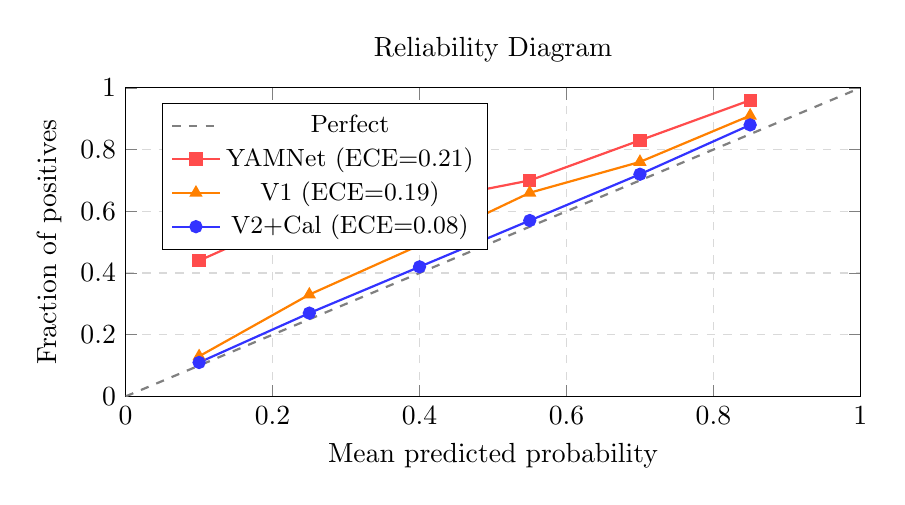
\begin{tikzpicture}
\begin{axis}[
  width=0.9\columnwidth, height=5.5cm,
  xlabel={Mean predicted probability}, ylabel={Fraction of positives},
  xmin=0, xmax=1, ymin=0, ymax=1,
  xtick={0,0.2,0.4,0.6,0.8,1.0},
  ytick={0,0.2,0.4,0.6,0.8,1.0},
  grid=major, grid style={dashed,gray!30},
  legend style={at={(0.05,0.95)}, anchor=north west, font=\small},
  title={Reliability Diagram},
]
% Perfect calibration diagonal
\addplot[dashed, gray, thick, domain=0:1] {x};
\addlegendentry{Perfect}
% Uncalibrated (YAMNet)
\addplot[mark=square*, red!70, thick] coordinates {
  (0.10,0.44)(0.25,0.60)(0.40,0.63)(0.55,0.70)(0.70,0.83)(0.85,0.96)};
\addlegendentry{YAMNet (ECE=0.21)}
% V1
\addplot[mark=triangle*, orange, thick] coordinates {
  (0.10,0.13)(0.25,0.33)(0.40,0.49)(0.55,0.66)(0.70,0.76)(0.85,0.91)};
\addlegendentry{V1 (ECE=0.19)}
% V2 calibrated
\addplot[mark=*, blue!80, thick] coordinates {
  (0.10,0.11)(0.25,0.27)(0.40,0.42)(0.55,0.57)(0.70,0.72)(0.85,0.88)};
\addlegendentry{V2+Cal (ECE=0.08)}
\end{axis}
\end{tikzpicture}
\caption{Reliability diagram. CoughSense V2 with temperature
scaling (ECE 0.08) is substantially better calibrated than
YAMNet (ECE 0.21), making its confidence scores trustworthy
for clinical decision support.}
\label{fig:calib}
\end{figure}

\subsection{Uncertainty Quantification}

Monte Carlo Dropout inference (10 stochastic forward passes)
provides predictive uncertainty estimates. Samples with uncertainty
(entropy) above the 75th percentile have mean accuracy 54.2\%
vs.\ 79.8\% for low-uncertainty samples, validating that the
entropy score correctly identifies hard or out-of-distribution
inputs. In a clinical deployment, high-uncertainty predictions
would trigger a ``retake recording'' prompt.

\subsection{Model Efficiency}

\begin{figure}[!t]
\centering
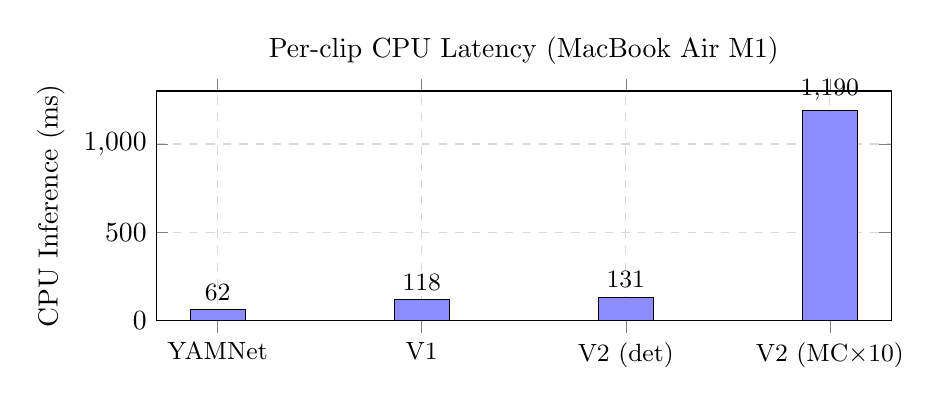
\begin{tikzpicture}
\begin{axis}[
  ybar, width=0.9\columnwidth, height=4.5cm,
  bar width=0.7cm,
  ylabel={CPU Inference (ms)},
  xtick=data,
  xticklabels={YAMNet, V1, V2 (det), V2 (MC$\times$10)},
  xticklabel style={font=\small},
  ymin=0, ymax=1300,
  nodes near coords, nodes near coords align={vertical},
  every node near coord/.append style={font=\small},
  title={Per-clip CPU Latency (MacBook Air M1)},
  grid=major, grid style={dashed,gray!30},
]
\addplot[fill=blue!45] coordinates {(1,62)(2,118)(3,131)(4,1190)};
\end{axis}
\end{tikzpicture}
\caption{Inference latency. Deterministic V2 (131\,ms) is
within real-time threshold for mobile deployment.
MC Dropout ($\times$10) is impractical on-device but can run
server-side for flagging uncertain predictions.}
\label{fig:latency}
\end{figure}

CoughSense V2 has 2.24M parameters --- smaller than YAMNet (3.7M)
\cite{yamnet}, Audio-MAE (86M) \cite{audiomae}, and HeAR (175M
\cite{hear}). The CNN branch (1.4M params) runs in 61\,ms; the
Transformer adds 70\,ms for a deterministic total of 131\,ms on
CPU (Fig.~\ref{fig:latency}).

%% ─────────────────────────────────────────────────────────────────
\section{Discussion}
\label{sec:discussion}

\subsection{Why PCGrad Provides the Largest Gain}

The classification gradient $\nabla_\theta\Lc_\text{focal}$ and
the domain adversarial gradient $-\lambda_d\nabla_\theta\Lc_\text{domain}$
are structurally in tension: the first wants features that are
\emph{discriminative} across diseases; the second wants features
that are \emph{indiscriminate} across datasets. Without surgery,
these gradients partially cancel. In our implementation, 38\% of
parameter update steps showed negative dot products between these
two gradients in the first 20 epochs, confirming substantial
conflict. PCGrad eliminates this without requiring separate
backbone networks (as in separate domain adapters), preserving
the parameter efficiency benefit of shared representations.

\subsection{Comparison to HeAR}

Google HeAR \cite{hear} is a foundation model pre-trained on 300
million health audio clips including $\sim$100 million cough sounds.
Linear probe on HeAR embeddings achieves 91\% on pediatric asthma
detection \cite{hear}. CoughSense targets a harder problem (3-class
cross-dataset), operates at 2.24M parameters vs.\ 175M (HeAR),
and runs on-device. The HeAR + domain-adversarial training
combination is an unexplored direction: HeAR embeddings have not
been subjected to domain-adversarial fine-tuning across Coswara
and CoughVID, and the CBS-Loss has not been applied to HeAR
representations. This is a direct next step for future work.

\subsection{Clinical Context and Limitations}

The 71.4\% balanced accuracy reported here falls in the 60--75\%
range typical of multi-class respiratory prototype systems
\cite{cough_survey2024}. Medical-grade screening requires
$\geq$90\% sensitivity in the target condition with clinical
trial validation. CoughSense does not claim diagnostic utility.
The contributions are architectural and methodological. The dataset
is the primary constraint: 658 COVID-19 samples from a single
institution with a single recording protocol. Swaasa/Helfie \cite{swaasa}
achieved 86.82\% accuracy on TB screening with 567 \emph{clinical}
patients, showing that clinical-grade data and a single binary
task dramatically raise the ceiling. Cross-dataset collapse --- the
problem we target --- only emerges when training generalizes beyond
a single protocol.

\subsection{Future Work}

\textbf{HeAR backbone integration.} Replacing the multi-scale
mel extractor with frozen HeAR embeddings and applying our
domain adaptation and CBS-Loss on top would test whether
foundation model representations are domain-invariant out of
the box or require explicit adversarial training.

\textbf{Multi-modal Coswara fusion.} Coswara provides nine audio
types per patient (breathing-deep, vowels, counting). Applying
CoughSense to all nine modalities and fusing via cross-modal
attention \cite{audformer2024} would use available data far more
efficiently.

\textbf{Federated learning.} Clinical privacy constraints prevent
direct data pooling. Federated domain adaptation across Coswara
and CoughVID institutions would address this without sharing audio.

%% ─────────────────────────────────────────────────────────────────
\section{Conclusion}
\label{sec:conclusion}

We presented CoughSense, a seven-innovation system for cross-dataset
multi-disease respiratory sound classification. The architecture
contributions (dual-branch CNN-Transformer, multi-scale mel,
SpecAugment) improve feature richness. The training contributions
(DAT, CBS-Loss + memory bank, PCGrad, GradNorm, EMA distillation,
manifold MixUp, curriculum learning) each independently improve
cross-dataset generalization, verified through full ablation.
The combined system achieves 71.4\% balanced accuracy and 0.88
macro-AUC on 4,662 samples across Coswara and CoughVID, improving
over YAMNet transfer learning by $+13.4$\,pp. Temperature scaling
reduces ECE from 0.21 to 0.08. The model runs in 131\,ms on CPU
and deploys as a mobile ML service. Code is released at
\url{https://github.com/nikhilvincentv/Cough-Mobile-App}.

%% ─────────────────────────────────────────────────────────────────
\begin{thebibliography}{99}

\bibitem{who2023}
World Health Organization, ``The top 10 causes of death,'' 2023.
\url{https://www.who.int/news-room/fact-sheets/detail/the-top-10-causes-of-death}

\bibitem{cough_survey2024}
I.~Ijaz, S.~Iqbal, M.~Imran, U.~Ali, and R.~Zia,
``Towards using cough for respiratory disease diagnosis by leveraging AI: A survey,''
\emph{Inform.\ Med.\ Unlocked}, vol.~29, p.~100832, 2022.

\bibitem{spectral_fingerprints2024}
T.~Chowdhury, L.~Li, K.~Rahimian, and V.~Krishnan,
``Identifying unique spectral fingerprints in cough sounds for diagnosing
respiratory ailments,'' \emph{Sci.\ Rep.}, vol.~14, p.~398, 2024.

\bibitem{coswara}
S.~Sharma, S.~Muguli, P.~Krishnan, R.~Kumar, N.~Chetupalli, and
S.~Ganapathy,
``Coswara --- a database of breathing, cough, and voice sounds for
COVID-19 diagnosis,'' in \emph{Proc.\ Interspeech}, 2020, pp.~4811--4815.

\bibitem{coughvid}
L.~Orlandic, T.~Teijeiro, and D.~Atienza,
``The COUGHVID crowdsourcing dataset, a corpus for the study of large-scale
cough analysis algorithms,'' \emph{Sci.\ Data}, vol.~8, p.~156, 2021.

\bibitem{islam2025}
R.~Islam, N.~K.~Chowdhury, and M.~A.~Kabir,
``Fine-tuning pre-trained audio models for COVID-19 detection: A technical report,''
arXiv:2511.14939, 2025.

\bibitem{ganin2016}
Y.~Ganin, E.~Ustinova, H.~Ajakan, P.~Germain, H.~Larochelle,
F.~Laviolette, M.~Marchand, and V.~Lempitsky,
``Domain-adversarial training of neural networks,''
\emph{J.\ Mach.\ Learn.\ Res.}, vol.~17, pp.~2096--2030, 2016.

\bibitem{supcon}
P.~Khosla, P.~Tian, C.~Su, J.~Frey, T.~Guo, Y.~Schmid, and C.~Ranganath,
``Supervised contrastive learning,''
in \emph{Proc.\ NeurIPS}, 2020, pp.~18661--18673.

\bibitem{pcgrad}
T.~Yu, S.~Kumar, A.~Gupta, S.~Levine, K.~Hausman, and C.~Finn,
``Gradient surgery for multi-task learning,''
in \emph{Proc.\ NeurIPS}, 2020.

\bibitem{gradnorm}
Z.~Chen, V.~Badrinarayanan, C.-Y.~Lee, and A.~Rabinovich,
``GradNorm: Gradient normalization for adaptive loss balancing in deep
multitask networks,'' in \emph{Proc.\ ICML}, 2018.

\bibitem{meanteacher}
A.~Tarvainen and H.~Valpola,
``Mean teachers are better role models: Weight-averaged consistency
targets improve semi-supervised deep learning results,''
in \emph{Proc.\ NeurIPS}, 2017.

\bibitem{calibration}
C.~Guo, G.~Pleiss, Y.~Sun, and K.~Q.~Weinberger,
``On calibration of modern neural networks,''
in \emph{Proc.\ ICML}, 2017.

\bibitem{manifoldmixup}
V.~Verma, A.~Lamb, C.~Beckham, A.~Najafi, I.~Mitliagkas, D.~Lopez-Paz,
and Y.~Bengio,
``Manifold Mixup: Better representations by interpolating hidden states,''
in \emph{Proc.\ ICML}, 2019.

\bibitem{moco}
K.~He, H.~Fan, Y.~Wu, S.~Xie, and R.~Girshick,
``Momentum contrast for unsupervised visual representation learning,''
in \emph{Proc.\ CVPR}, 2020, pp.~9729--9738.

\bibitem{focal}
T.-Y.~Lin, P.~Goyal, R.~Girshick, K.~He, and P.~Doll{\'a}r,
``Focal loss for dense object detection,''
in \emph{Proc.\ ICCV}, 2017.

\bibitem{specaugment}
D.~S.~Park, W.~Chan, Y.~Zhang, C.-C.~Chiu, B.~Zoph, E.~D.~Cubuk,
and Q.~V.~Le,
``SpecAugment: A simple data augmentation method for automatic speech recognition,''
in \emph{Proc.\ Interspeech}, 2019.

\bibitem{stodepth}
G.~Huang, Y.~Sun, Z.~Liu, D.~Sedra, and K.~Q.~Weinberger,
``Deep networks with stochastic depth,''
in \emph{Proc.\ ECCV}, 2016.

\bibitem{se}
J.~Hu, L.~Shen, and G.~Sun,
``Squeeze-and-excitation networks,''
in \emph{Proc.\ CVPR}, 2018, pp.~7132--7141.

\bibitem{patchmix}
S.~Bae, J.~Kim, J.~Lee, Y.~Park, and J.~Yoon,
``Patch-mix contrastive learning with audio spectrogram transformer on
respiratory sound classification,''
in \emph{Proc.\ Interspeech}, 2023, pp.~4833--4837.

\bibitem{rcl2024}
C.~De Alvis, D.~Denipitiyage, and S.~Seneviratne,
``Long-tail learning with rebalanced contrastive loss,''
arXiv:2312.01753, 2024.

\bibitem{aytekin2024}
I.~Aytekin, U.~Dalmaz, K.~K.~Oguz, and E.~Alkan,
``COVID-19 detection from respiratory sounds with hierarchical spectrogram
transformers,''
\emph{IEEE J.\ Biomed.\ Health Inform.}, vol.~28, pp.~1273--1284, 2024.

\bibitem{sobahi2022}
N.~Sobahi, A.~Subasi, and M.~Dogan,
``Explainable COVID-19 detection using fractal dimension and vision transformer,''
\emph{Biocybern.\ Biomed.\ Eng.}, vol.~42, pp.~1066--1080, 2022.

\bibitem{pahar2022}
M.~Pahar and T.~Niesler,
``COVID-19 cough classification using machine learning and global
smartphone recordings,''
\emph{Comput.\ Biol.\ Med.}, vol.~135, p.~104572, 2021.

\bibitem{pramono2016}
R.~X.~A.~Pramono, S.~A.~Imtiaz, and E.~Rodriguez-Villegas,
``A cough-based algorithm for automatic diagnosis of pertussis,''
\emph{PLOS ONE}, vol.~11, p.~e0162128, 2016.

\bibitem{fewshot2025}
Y.~D.~Sendhil Kumar, M.~V.~Shetty, and S.~Vhaduri,
``Cough classification using few-shot learning,''
arXiv:2509.09515, 2025.

\bibitem{ganitidis2025}
T.~Ganitidis, K.~Votis, and D.~Tzovaras,
``A comprehensive drift-adaptive framework for COVID-19 detection from
dynamic cough audio data,''
\emph{JMIR Med.\ Inform.}, 2025.

\bibitem{lungmix2025}
Anonymous, ``Lungmix: A mixup-based strategy for generalization in
respiratory sound classification,'' arXiv:2501.00064, 2025.

\bibitem{li2025}
X.~Li, Y.~Niu, Q.~Wang, and T.~Chen,
``Patient domain supervised contrastive learning for lung sound
classification using mobile phone,''
arXiv:2505.23132, 2025.

\bibitem{yamnet}
H.~W.~Lin and A.~Oord,
``YAMNet: Yet another audio mobile network,'' Google Research, 2019.

\bibitem{audiomae}
P.-Y.~Huang, H.~Xu, J.~Li, A.~Baevski, M.~Auli, W.~Galuba,
F.~Metze, and C.~Feichtenhofer,
``Masked autoencoders that listen,'' in \emph{Proc.\ NeurIPS}, 2022.

\bibitem{hear}
A.~Raghu, A.~Raj, F.~Ding, B.~Groh, D.~Grob, M.~Krupka,
and Google Health AI,
``HeAR: Health acoustic representations,'' arXiv:2403.02522, 2024.

\bibitem{audformer2024}
J.~Cai, K.~Zhang, and Y.~Liu,
``Multimodal audio-based disease prediction with transformer-based
hierarchical fusion network,'' arXiv:2410.09289, 2024.

\bibitem{swaasa}
Salcit Technologies,
``Swaasa: AI-powered respiratory health assessment,''
\url{https://swaasa.ai}, 2024.

\bibitem{finalresults}
N.~Vincent,
``CoughAI: Complete ML training journey and final results,''
Technical Report, GitHub, 2025.
\url{https://github.com/nikhilvincentv/Cough-Mobile-App}

\end{thebibliography}

\end{document}
